% Source: graduate-coursework/Research/Intro_to_Agents/handouts/Part7_Parallelization.tex

\documentclass[border=4pt]{standalone}
\usepackage{amsmath,amssymb,amsfonts}
\usepackage[T1]{fontenc}
\usepackage{graphicx}
\usepackage{lmodern}
\usepackage{tikz}
\usepackage{xcolor}
\usetikzlibrary{shapes.geometric, arrows.meta, positioning, calc, fit, backgrounds, matrix, decorations.pathreplacing}

\definecolor{UofSCGarnet}{HTML}{73000a}
\definecolor{UofSCBlack}{HTML}{000000}
\definecolor{UofSCWhite}{HTML}{ffffff}
\definecolor{UofSCRose}{HTML}{CC2E40}
\definecolor{UofSCAtlantic}{HTML}{466A9F}
\definecolor{UofSCCongaree}{HTML}{1F414D}
\definecolor{UofSCHorseshoe}{HTML}{65780B}
\definecolor{UofSCGrass}{HTML}{CED318}
\definecolor{UofSCHoneycomb}{HTML}{A49137}
\definecolor{UofSC90Black}{HTML}{363636}
\definecolor{UofSC70Black}{HTML}{5C5C5C}
\definecolor{UofSC50Black}{HTML}{A2A2A2}
\definecolor{UofSCWarmGrey}{HTML}{676156}
\definecolor{UofSCSandstorm}{HTML}{FFF2E3}
\definecolor{UofSCDarkGarnet}{HTML}{570008}
\definecolor{UofSCAzalea}{HTML}{844247}

\tikzset{
    % Node styles - all with sharp corners
    agentbox/.style={
        rectangle,
        draw=UofSCGarnet,
        fill=UofSCSandstorm,
        thick,
        minimum width=2cm,
        minimum height=0.8cm,
        text centered,
        font=\footnotesize
    },
    processbox/.style={
        rectangle,
        draw=UofSCAtlantic,
        fill=UofSCWhite,
        thick,
        minimum width=2.5cm,
        minimum height=0.7cm,
        text centered,
        font=\footnotesize
    },
    syncbox/.style={
        rectangle,
        draw=UofSCCongaree,
        fill=UofSCCongaree!20,
        thick,
        minimum width=3cm,
        minimum height=0.5cm,
        text centered,
        font=\footnotesize\bfseries
    },
    resultbox/.style={
        rectangle,
        draw=UofSCHorseshoe,
        fill=UofSCGrass!30,
        thick,
        minimum width=2cm,
        minimum height=0.7cm,
        text centered,
        font=\footnotesize
    },
    % Arrow styles
    myarrow/.style={
        ->,
        >=Stealth,
        thick,
        UofSCBlack
    },
    dashedarrow/.style={
        ->,
        >=Stealth,
        thick,
        dashed,
        UofSC70Black
    },
    % Timeline styles
    timeline/.style={
        draw=UofSCBlack,
        thick,
        ->,
        >=Stealth
    },
    timeblock/.style={
        rectangle,
        draw=none,
        minimum height=0.5cm,
        text centered,
        font=\tiny
    }
}

\begin{document}
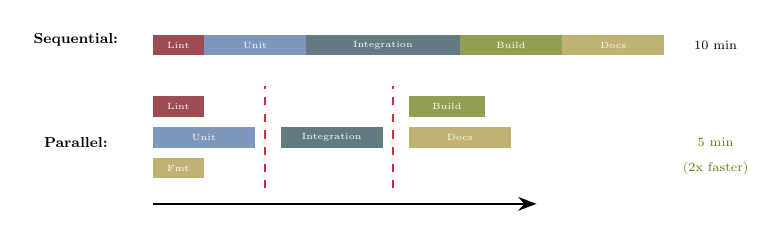
\begin{tikzpicture}[scale=0.65, transform shape]
            % Sequential comparison (top)
            \node[font=\footnotesize\bfseries] at (-1,3.5) {Sequential:};

            \fill[UofSCGarnet!70] (0.5,3.2) rectangle (1.5,3.6);
            \fill[UofSCAtlantic!70] (1.5,3.2) rectangle (3.5,3.6);
            \fill[UofSCCongaree!70] (3.5,3.2) rectangle (6.5,3.6);
            \fill[UofSCHorseshoe!70] (6.5,3.2) rectangle (8.5,3.6);
            \fill[UofSCHoneycomb!70] (8.5,3.2) rectangle (10.5,3.6);

            \node[font=\tiny,white] at (1,3.4) {Lint};
            \node[font=\tiny,white] at (2.5,3.4) {Unit};
            \node[font=\tiny,white] at (5,3.4) {Integration};
            \node[font=\tiny,white] at (7.5,3.4) {Build};
            \node[font=\tiny,white] at (9.5,3.4) {Docs};

            \node[font=\scriptsize] at (11.5,3.4) {10 min};

            % Parallel (bottom)
            \node[font=\footnotesize\bfseries] at (-1,1.5) {Parallel:};

            % Phase 1
            \fill[UofSCGarnet!70] (0.5,2) rectangle (1.5,2.4);
            \fill[UofSCAtlantic!70] (0.5,1.4) rectangle (2.5,1.8);
            \fill[UofSCHoneycomb!70] (0.5,0.8) rectangle (1.5,1.2);

            \node[font=\tiny,white] at (1,2.2) {Lint};
            \node[font=\tiny,white] at (1.5,1.6) {Unit};
            \node[font=\tiny,white] at (1,1) {Fmt};

            % Sync line
            \draw[thick,dashed,UofSCRose] (2.7,0.6) -- (2.7,2.6);

            % Phase 2
            \fill[UofSCCongaree!70] (3,1.4) rectangle (5,1.8);
            \node[font=\tiny,white] at (4,1.6) {Integration};

            % Sync line
            \draw[thick,dashed,UofSCRose] (5.2,0.6) -- (5.2,2.6);

            % Phase 3
            \fill[UofSCHorseshoe!70] (5.5,2) rectangle (7,2.4);
            \fill[UofSCHoneycomb!70] (5.5,1.4) rectangle (7.5,1.8);

            \node[font=\tiny,white] at (6.25,2.2) {Build};
            \node[font=\tiny,white] at (6.5,1.6) {Docs};

            \node[font=\scriptsize,UofSCHorseshoe] at (11.5,1.5) {5 min};
            \node[font=\scriptsize,UofSCHorseshoe] at (11.5,1) {(2x faster)};

            % Timeline
            \draw[timeline] (0.5,0.3) -- (8,0.3);
        \end{tikzpicture}
\end{document}
